% Nguồn SGK Toán 9 Tập hai — Chương VIII, Luyện tập chung sau Bài 26, trang 64--65:
% https://cdn3.olm.vn/upload/thuvienso/4491669493-page-64-1771844555729.png
% https://cdn3.olm.vn/upload/thuvienso/4491669493-page-65-1771844556047.png

\section*{Luyện tập chung}

\begin{exercises}
    \textbf{Ví dụ}

    Tấm bìa cứng A hình tròn được chia thành 3 hình quạt có diện tích bằng nhau,
    đánh số 1; 2; 3 và tấm bìa cứng B hình tròn được chia thành 5 hình quạt có diện tích
    bằng nhau, đánh số 1; 2; 3; 4; 5 (H.8.3). Trục quay của A và B được gắn mũi tên ở
    tâm. Bạn Nam quay tấm bìa A, bạn Bình quay tấm bìa B. Quan sát xem mũi tên dừng
    ở hình quạt nào trên hai tấm bìa.

    \begin{center}
        \begin{tikzpicture}[line join=round,line cap=round]
            \coordinate (OA) at (0,0);
            \coordinate (OB) at (4.4,0);

            % Tấm bìa A: ba hình quạt bằng nhau như Hình 8.3.
            \path[fill=cyan!45!black,draw=black!65]
                (OA) -- ++(0:1.35) arc[start angle=0,end angle=120,radius=1.35] -- cycle;
            \path[fill=red!75!orange,draw=black!65]
                (OA) -- ++(120:1.35) arc[start angle=120,end angle=240,radius=1.35] -- cycle;
            \path[fill=orange!85,draw=black!65]
                (OA) -- ++(240:1.35) arc[start angle=240,end angle=360,radius=1.35] -- cycle;
            \node[text=white,font=\bfseries] at ($(OA)+(60:0.76)$) {2};
            \node[text=white,font=\bfseries] at ($(OA)+(180:0.76)$) {1};
            \node[text=white,font=\bfseries] at ($(OA)+(300:0.76)$) {3};
            \draw[white,line width=1.5pt,-{Stealth[length=2.5mm,width=2mm]}]
                (OA) -- ($(OA)+(270:0.84)$);
            \node[below=5pt of OA,yshift=-1.35cm] {Tấm bìa A};

            % Tấm bìa B: năm hình quạt bằng nhau như Hình 8.3.
            \path[fill=red!75!orange,draw=black!65]
                (OB) -- ++(90:1.35) arc[start angle=90,end angle=162,radius=1.35] -- cycle;
            \path[fill=blue!70,draw=black!65]
                (OB) -- ++(18:1.35) arc[start angle=18,end angle=90,radius=1.35] -- cycle;
            \path[fill=green!55!black,draw=black!65]
                (OB) -- ++(-54:1.35) arc[start angle=-54,end angle=18,radius=1.35] -- cycle;
            \path[fill=violet!80,draw=black!65]
                (OB) -- ++(-126:1.35) arc[start angle=-126,end angle=-54,radius=1.35] -- cycle;
            \path[fill=orange!85,draw=black!65]
                (OB) -- ++(-198:1.35) arc[start angle=-198,end angle=-126,radius=1.35] -- cycle;
            \node[text=white,font=\bfseries] at ($(OB)+(126:0.76)$) {1};
            \node[text=white,font=\bfseries] at ($(OB)+(54:0.76)$) {2};
            \node[text=white,font=\bfseries] at ($(OB)+(-18:0.76)$) {3};
            \node[text=white,font=\bfseries] at ($(OB)+(-90:0.76)$) {4};
            \node[text=white,font=\bfseries] at ($(OB)+(-162:0.76)$) {5};
            \draw[white,line width=1.5pt,-{Stealth[length=2.5mm,width=2mm]}]
                (OB) -- ($(OB)+(-90:0.84)$);
            \node[below=5pt of OB,yshift=-1.35cm] {Tấm bìa B};
        \end{tikzpicture}

        \textit{Hình 8.3}
    \end{center}

    \begin{enumerate}[label=\alph*)]
        \item Phép thử là gì?
        \item Mô tả không gian mẫu của phép thử.
        \item Tính xác suất của các biến cố sau:

        $E$: “Tích hai số ở hình quạt mà hai mũi tên chỉ vào bằng 6”;

        $F$: “Tích hai số ở hình quạt mà hai mũi tên chỉ vào nhỏ hơn 5”;

        $G$: “Tích hai số ở hình quạt mà hai mũi tên chỉ vào là số chẵn”.
    \end{enumerate}

    \textbf{Giải}

    \begin{enumerate}[label=\alph*)]
        \item Phép thử là bạn Nam quay tấm bìa A, bạn Bình quay tấm bìa B.

        \item Ta lập bảng sau:

        \begin{center}
            \begin{tblr}{
                colspec={Q[c,m] *{3}{Q[c,m]}},
                cells={valign=m},
                row{1}={bg=orange!12},
                column{1}={bg=yellow!15},
                cell{1}{1}={bg=yellow!15}
            }
                \begin{tikzpicture}[baseline=(current bounding box.center)]
                    \path[use as bounding box] (0,0) rectangle (3.2,1.35);
                    \draw (0,1.35) -- (3.2,0);
                    \node[anchor=north east,font=\footnotesize] at (3.1,1.27) {Tấm bìa A};
                    \node[anchor=south west,font=\footnotesize] at (0.1,0.08) {Tấm bìa B};
                \end{tikzpicture}
                & 1 & 2 & 3 \\
                1 & $(1, 1)$ & $(1, 2)$ & $(1, 3)$ \\
                2 & $(2, 1)$ & $(2, 2)$ & $(2, 3)$ \\
                3 & $(3, 1)$ & $(3, 2)$ & $(3, 3)$ \\
                4 & $(4, 1)$ & $(4, 2)$ & $(4, 3)$ \\
                5 & $(5, 1)$ & $(5, 2)$ & $(5, 3)$
            \end{tblr}
        \end{center}

        Mỗi ô trong bảng trên là một kết quả có thể. Các kết quả có thể này là đồng khả năng.

        Không gian mẫu là
        \[
            \begin{aligned}
                \Omega=\{&(1, 1); (1, 2); (1, 3); (2, 1); (2, 2); (2, 3); (3, 1); (3, 2);\\
                &(3, 3); (4, 1); (4, 2); (4, 3); (5, 1); (5, 2); (5, 3)\}.
            \end{aligned}
        \]

        Không gian mẫu có 15 phần tử.

        \item
        \begin{itemize}
            \item Có 2 kết quả thuận lợi cho biến cố $E$ là $(3, 2)$ và $(2, 3)$. Vậy $P(E)=\dfrac{2}{15}$.

            \item Các kết quả thuận lợi cho biến cố $F$: Có một ô có tích hai số bằng 1 là $(1, 1)$; các ô
            có tích hai số bằng 2 là $(1, 2)$; $(2, 1)$; các ô có tích hai số bằng 3 là $(1, 3)$; $(3, 1)$; các
            ô có tích hai số bằng 4 là $(2, 2)$; $(4, 1)$. Do đó, có 7 kết quả thuận lợi cho biến cố $F$
            là $(1, 1)$; $(1, 2)$; $(2, 1)$; $(1, 3)$; $(3, 1)$; $(2, 2)$; $(4, 1)$. Vậy $P(F)=\dfrac{7}{15}$.

            \item Tích $ab$ là số chẵn khi và chỉ khi trong cặp $(a, b)$ có ít nhất một số chẵn.
            Do đó, có 9 kết quả thuận lợi cho biến cố $G$ là $(1, 2)$; $(2, 1)$; $(2, 2)$; $(2, 3)$; $(3, 2)$; $(4, 1)$;
            $(4, 2)$; $(4, 3)$; $(5, 2)$.

            Vậy $P(G)=\dfrac{9}{15}=\dfrac{3}{5}$.
        \end{itemize}
    \end{enumerate}

    \subsection{Bài tập}

    \begin{questions}[resume=SGK]
        \item Có hai túi đựng các tấm thẻ. Túi I đựng 4 tấm thẻ ghi
        các chữ cái TT, TH, HT và HH. Túi II đựng 2 tấm thẻ
        ghi các chữ cái T và H. Từ mỗi túi rút ngẫu nhiên ra
        một tấm thẻ rồi ghép hai thẻ lại với nhau để được ba
        chữ cái, trong đó thẻ hai chữ cái đặt trước, chẳng hạn
        tấm thẻ TT ghép với tấm thẻ H được ba chữ cái TTH.
        Tính xác suất của các biến cố sau:

        \begin{center}
            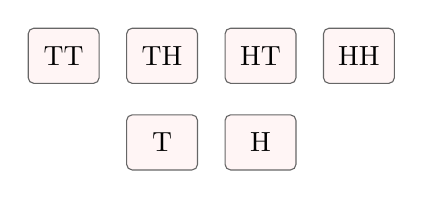
\begin{tikzpicture}
                \foreach \x/\label in {0/TT,1.25/TH,2.5/HT,3.75/HH}
                    \node[draw=black!60,rounded corners=2pt,fill=pink!15,minimum width=9mm,minimum height=7mm]
                        at (\x,0.55) {\label};
                \foreach \x/\label in {1.25/T,2.5/H}
                    \node[draw=black!60,rounded corners=2pt,fill=pink!15,minimum width=9mm,minimum height=7mm]
                        at (\x,-0.55) {\label};
            \end{tikzpicture}
        \end{center}

        \begin{questions}
            \item $E$: “Trong ba chữ cái, có hai chữ H và một chữ T”;

            \answerline
            \answerline

            \item $F$: “Trong ba chữ cái, có nhiều nhất hai chữ T”.

            \answerline
            \answerline
        \end{questions}

        \item Gieo đồng thời hai con xúc xắc cân đối và đồng chất I và II. Tính xác suất của các
        biến cố sau:

        $G$: “Không có con xúc xắc nào xuất hiện mặt 6 chấm”;

        \answerline
        \answerline

        $H$: “Số chấm xuất hiện trên con xúc xắc I là số lẻ và số chấm xuất hiện trên con
        xúc xắc II lớn hơn 4”;

        \answerline
        \answerline

        $K$: “Số chấm xuất hiện trên cả hai con xúc xắc lớn hơn 2”.

        \answerline
        \answerline

        \item Trên một dãy phố có ba quán ăn A, B, C. Hai bạn Văn và Hải mỗi người chọn ngẫu
        nhiên một quán ăn để ăn trưa.
        \begin{questions}
            \item Mô tả không gian mẫu của phép thử.

            \answerline
            \answerline

            \item Tính xác suất của các biến cố sau:

            $E$: “Hai bạn cùng vào một quán”;

            \answerline

            $F$: “Cả hai bạn không chọn quán C”;

            \answerline

            $G$: “Có ít nhất một bạn chọn quán B”.

            \answerline
        \end{questions}
    \end{questions}
\end{exercises}
